\section{Non-Preemptive Protocol}

In this section, I will explain about Non-Preemptive Protocol.

\subsection{Definition}

This protocol is a simple protocol and named non-preemptive(NP) because it avoids any interruption on running task $\tau_{j}$ that accessing a resource $ R_{k} $ that guarded by, $ S_{k} $. To reduce total blocking time experienced by the task $\tau_{i}$ that has the highest priority, this protocol just increases the priority of the task $\tau_{j}$ that currently accessing the resource $ R_{k} $, so that the task will not be interrupted and can be done much faster.Without this protocol, the task that highest priority $\tau_{i}$ will interrupt the task $\tau_{j}$ that currently accessing the resource $ R_{k} $ even though the task cannot access the resource because it already guarded by $ S_{k} $. The scheduler then switch back to the task before to finish its process, this switch context process could cause longer blocking time experienced by the highest priority task. After the task$\tau_{j}$ finishes accessing the resources, its priority will be back to its nominal priority $ P_{j} $. These situations can be compared through ``Fig. \ref{fig:An_example_of_priority_inversion}'' and ``Fig. \ref{fig:Example_of_NPP_preventing_priority_inversion}''. So, the priority of the task $\tau_{j}$that currently accessing the resource is 

\begin{equation}
\citeequation{p_{j}(R_{k})=\underset{h}{\mathrm{max}}\{P_{h}\}}{b5}\label{eq5}
\end{equation}

\begin{figure}[ht]
    \centering
    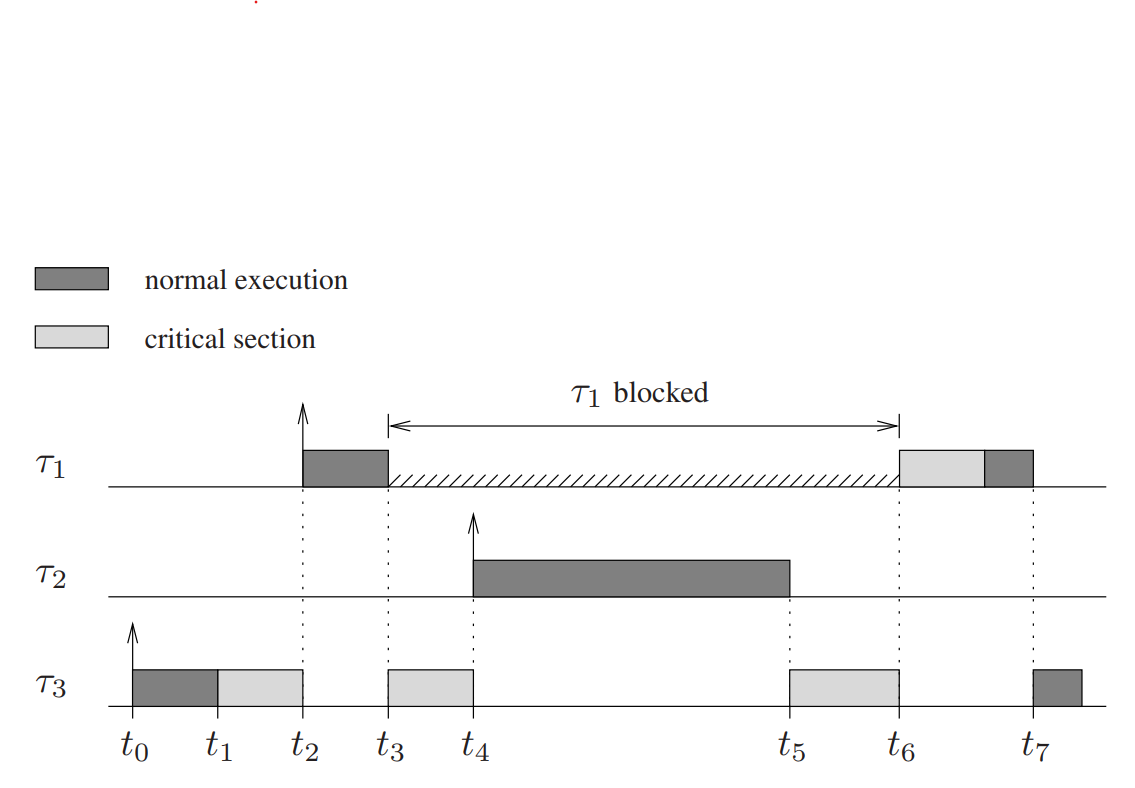
\includegraphics[width=0.5\textwidth]{An_example_of_priority_inversion}
    \caption{An example of priority inversion.. \cite{b5}}
    \label{fig:An_example_of_priority_inversion}
\end{figure}

\begin{figure}[ht]
    \centering
    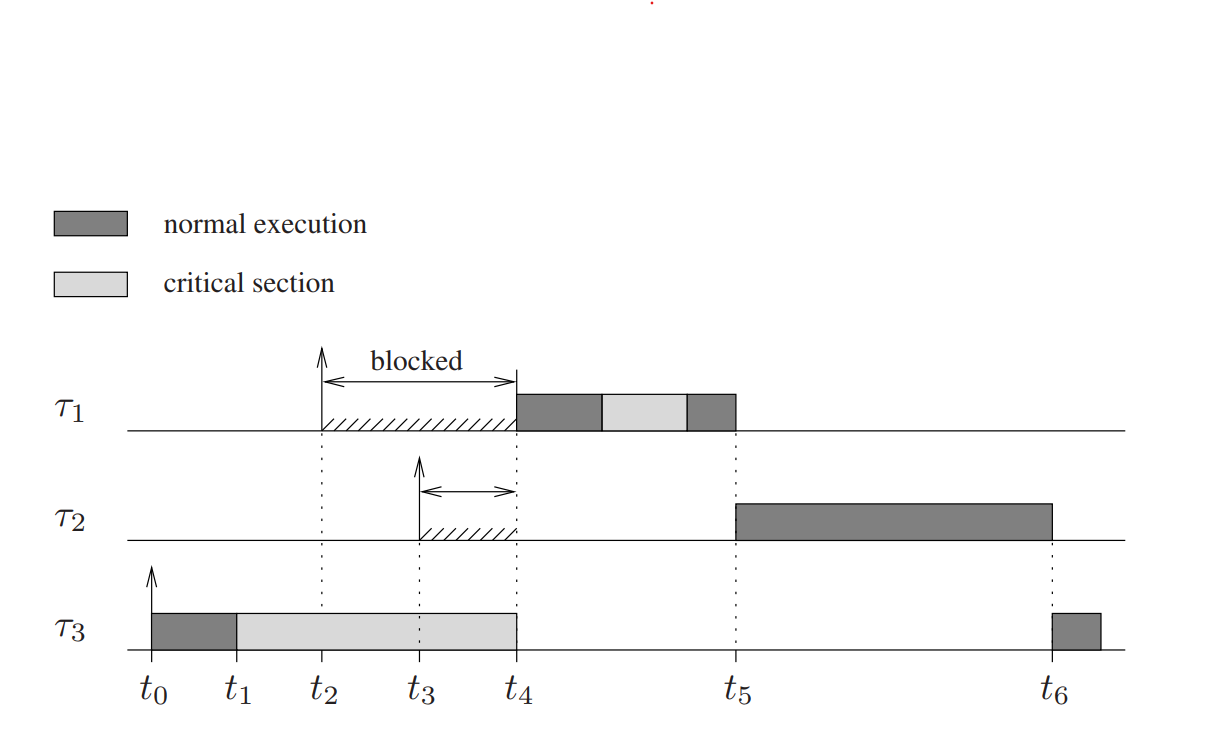
\includegraphics[width=0.5\textwidth]{Example_of_NPP_preventing_priority_inversion}
    \caption{Example of NPP preventing priority inversion. \cite{b5}}
    \label{fig:Example_of_NPP_preventing_priority_inversion}
\end{figure}


\subsection{Blocking time computation}

	The total of critical section of lower priority task $\tau_{j}$ blocking higher priority tasks $\tau_{i}$ is

\begin{equation}
\citeequation{ \gamma_{i}=\{Z_{j,k} | P_{j}<P_{i}, k=1,...,m \}}{b5}\label{eq6}
\end{equation}

From my understanding, the value of k could be more than one if the task that has the highest priority wants to access more than one resource and each resource is currently accessed by the task that has lower priority. Hence, in the total duration, the highest priority task is blocked is

\begin{equation}
\citeequation{B_{i}(R_{k})=\underset{j,k}{\mathrm{max}} \{ \delta_{j,k}-1 | Z_{j,k} \in \gamma_{i}\}}{b5}\label{eq7}
\end{equation}


The value of $\delta_{j,k}$is reduced one unit time because the task that has a lower priority, $\tau_{j}$ could block the task with the highest priority, $\tau_{i}$ from accessing a resource only and only if the task $\tau_{j}$  arrived at least one unit time earlier than $\tau_{i}$.

\subsection{Implementation Strategies}

As stated by \cite{b6}---``All commercial RTOSs have a means for beginning and ending a critical section. Invoking this Scheduler operation prevents all task switching from occurring during the critical section. If we write our own RTOS, the most common way to do this is to set the Disable Interrupts bit on our processor's flags register. The precise details of this vary, naturally, depending on the specific processor.". Means that, this resource access protocol is nothing more than avoiding interrupt on running task. 

Base on the model that I made using UPPAAL, it is true that the result in terms of the longest blocking time experienced by the highest priority task in both cases, disabling interrupt without NPP and enabling interrupt with NPP, is the same. Using the same model, I found that it is possible that a higher priority task could miss the deadline without applying NNP while interrupt is enabled. The model can be downloaded from \url{https://github.com/Adib6637/UPPAAL} to see the simulation.

\subsection{Sample Model}

In this section, I will explain the sample model of NPP that I made. For this sample model, I use a clock that can display time and date. Considering the task of displaying date,$\tau_{d}$ has higher priority than the task of displaying time,$\tau_{t}$ and they share the same resource which is Display unit,$R_{d}$, the scheduler will preempt the task $\tau_{t}$ whenever the task $\tau_{d}$ is ready as shown in ``Fig. \ref{fig:sample_model_without_npp}''.
\begin{figure}[ht]
    \centering
    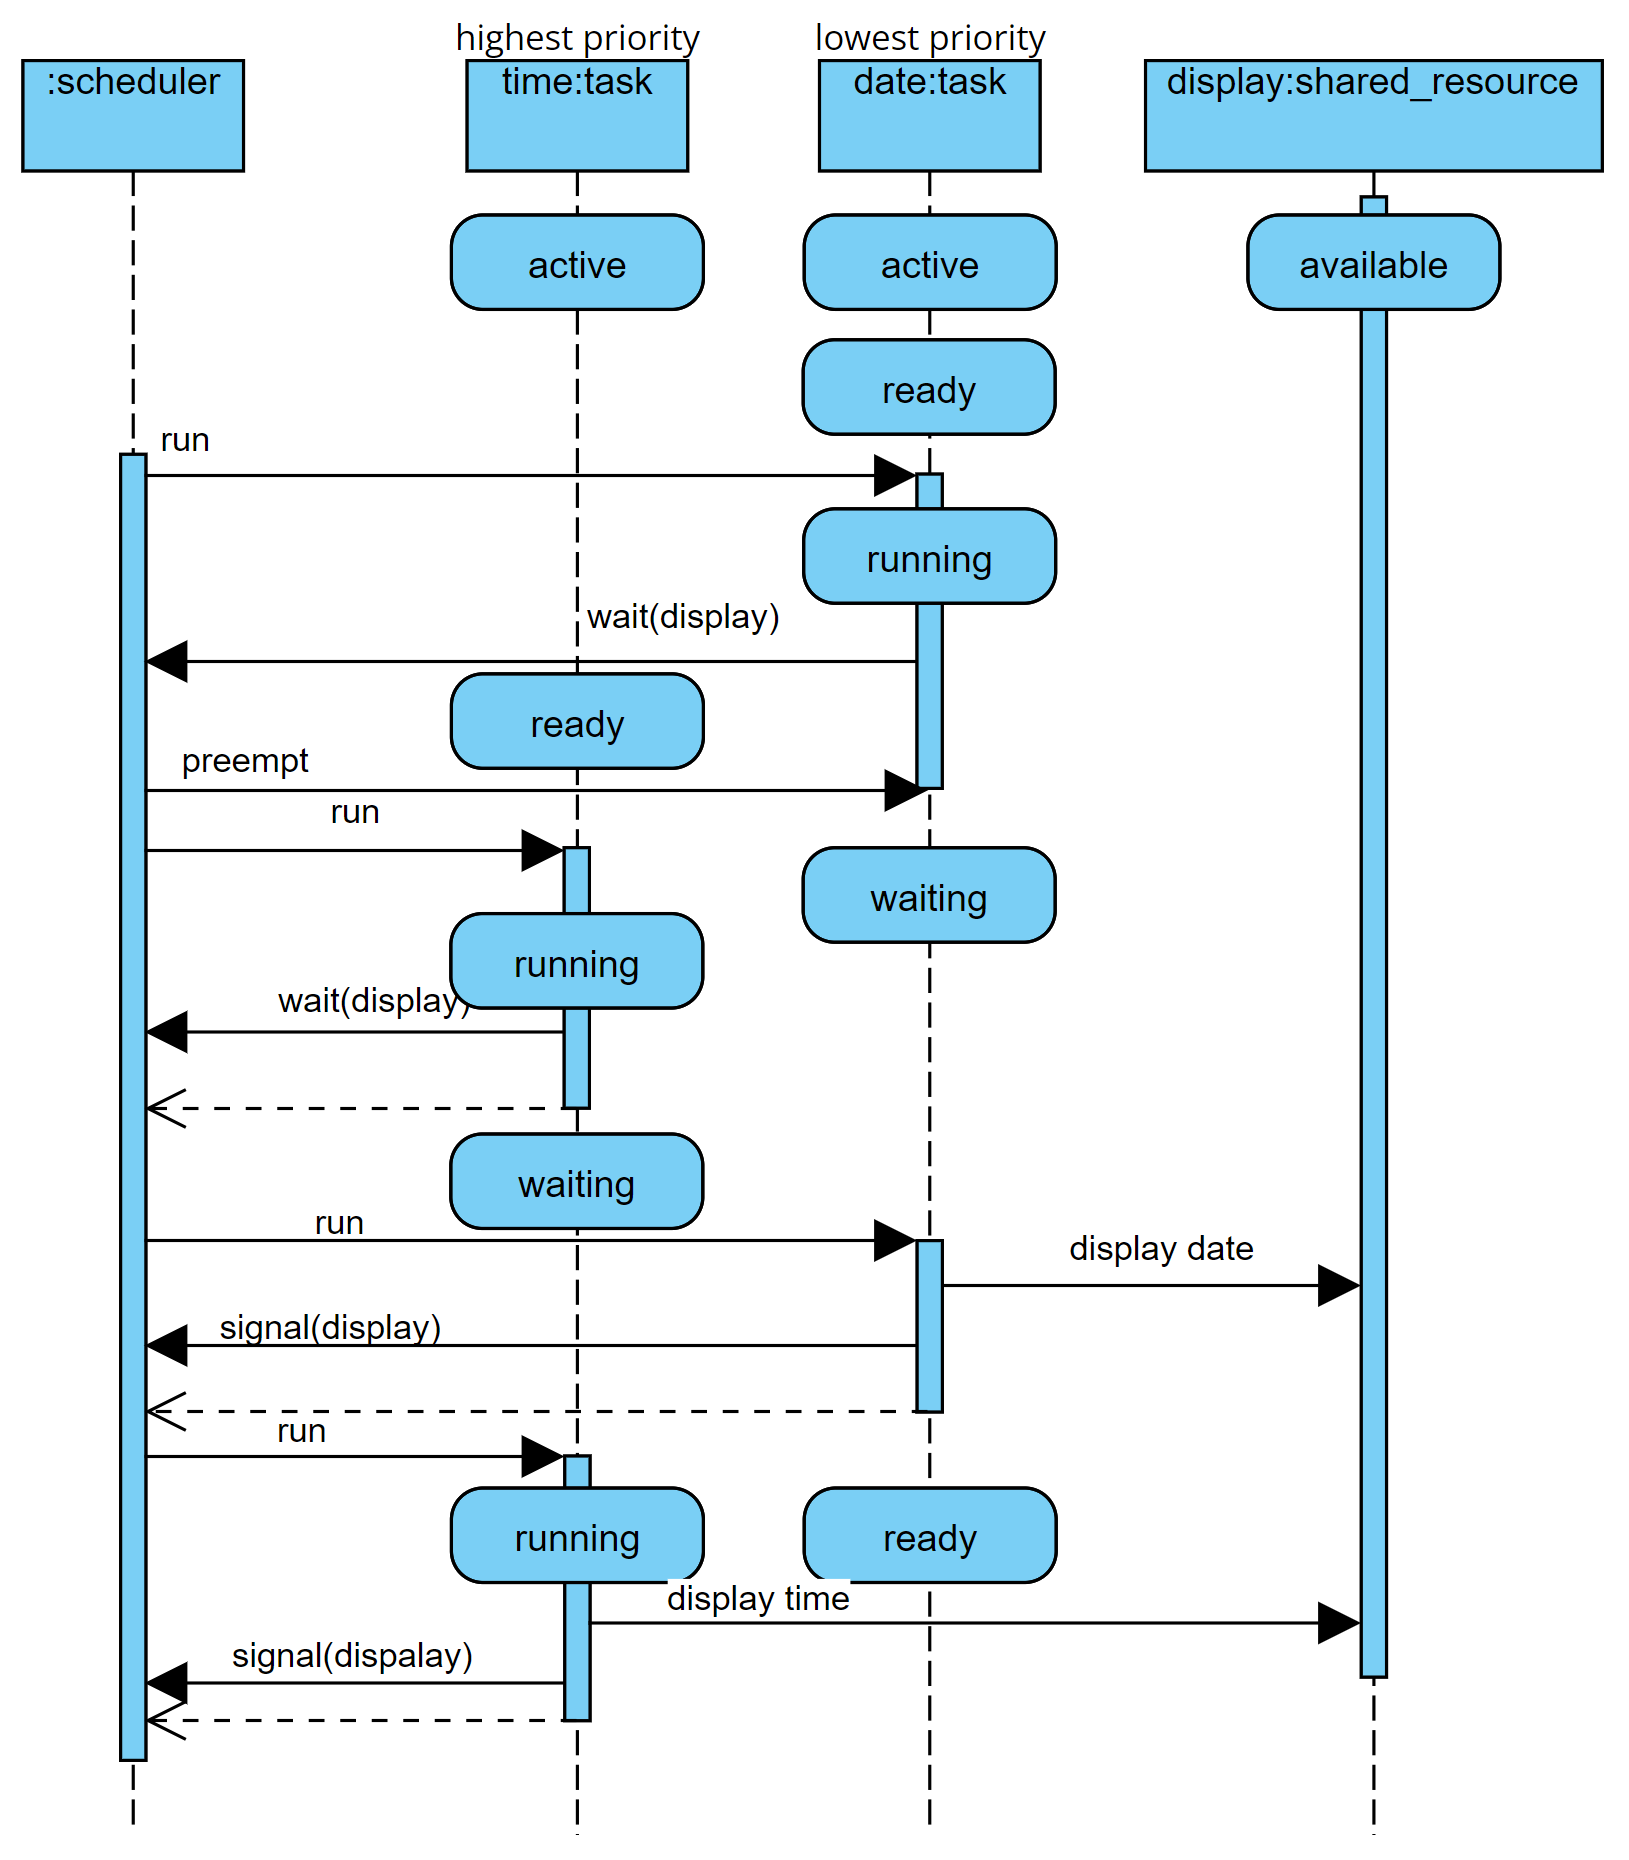
\includegraphics[width=0.5\textwidth]{sample_model_without_npp}
    \caption{Sample Model without Non-Preemptive Protocol} \cite{b6}
    \label{fig:sample_model_without_npp}
\end{figure}

By applying NNP as shown in ``Fig. \ref{fig:sample_model_with_npp}'', the task $\tau_{d}$ cannot be preempted in the event the task $\tau_{t}$ is ready because the dynamic priority of the task $\tau_{d}$ is arisen to the highest and back to its nominal value when the task $\tau_{d}$ leaves its critical section. 


\begin{figure}[ht]
    \centering
    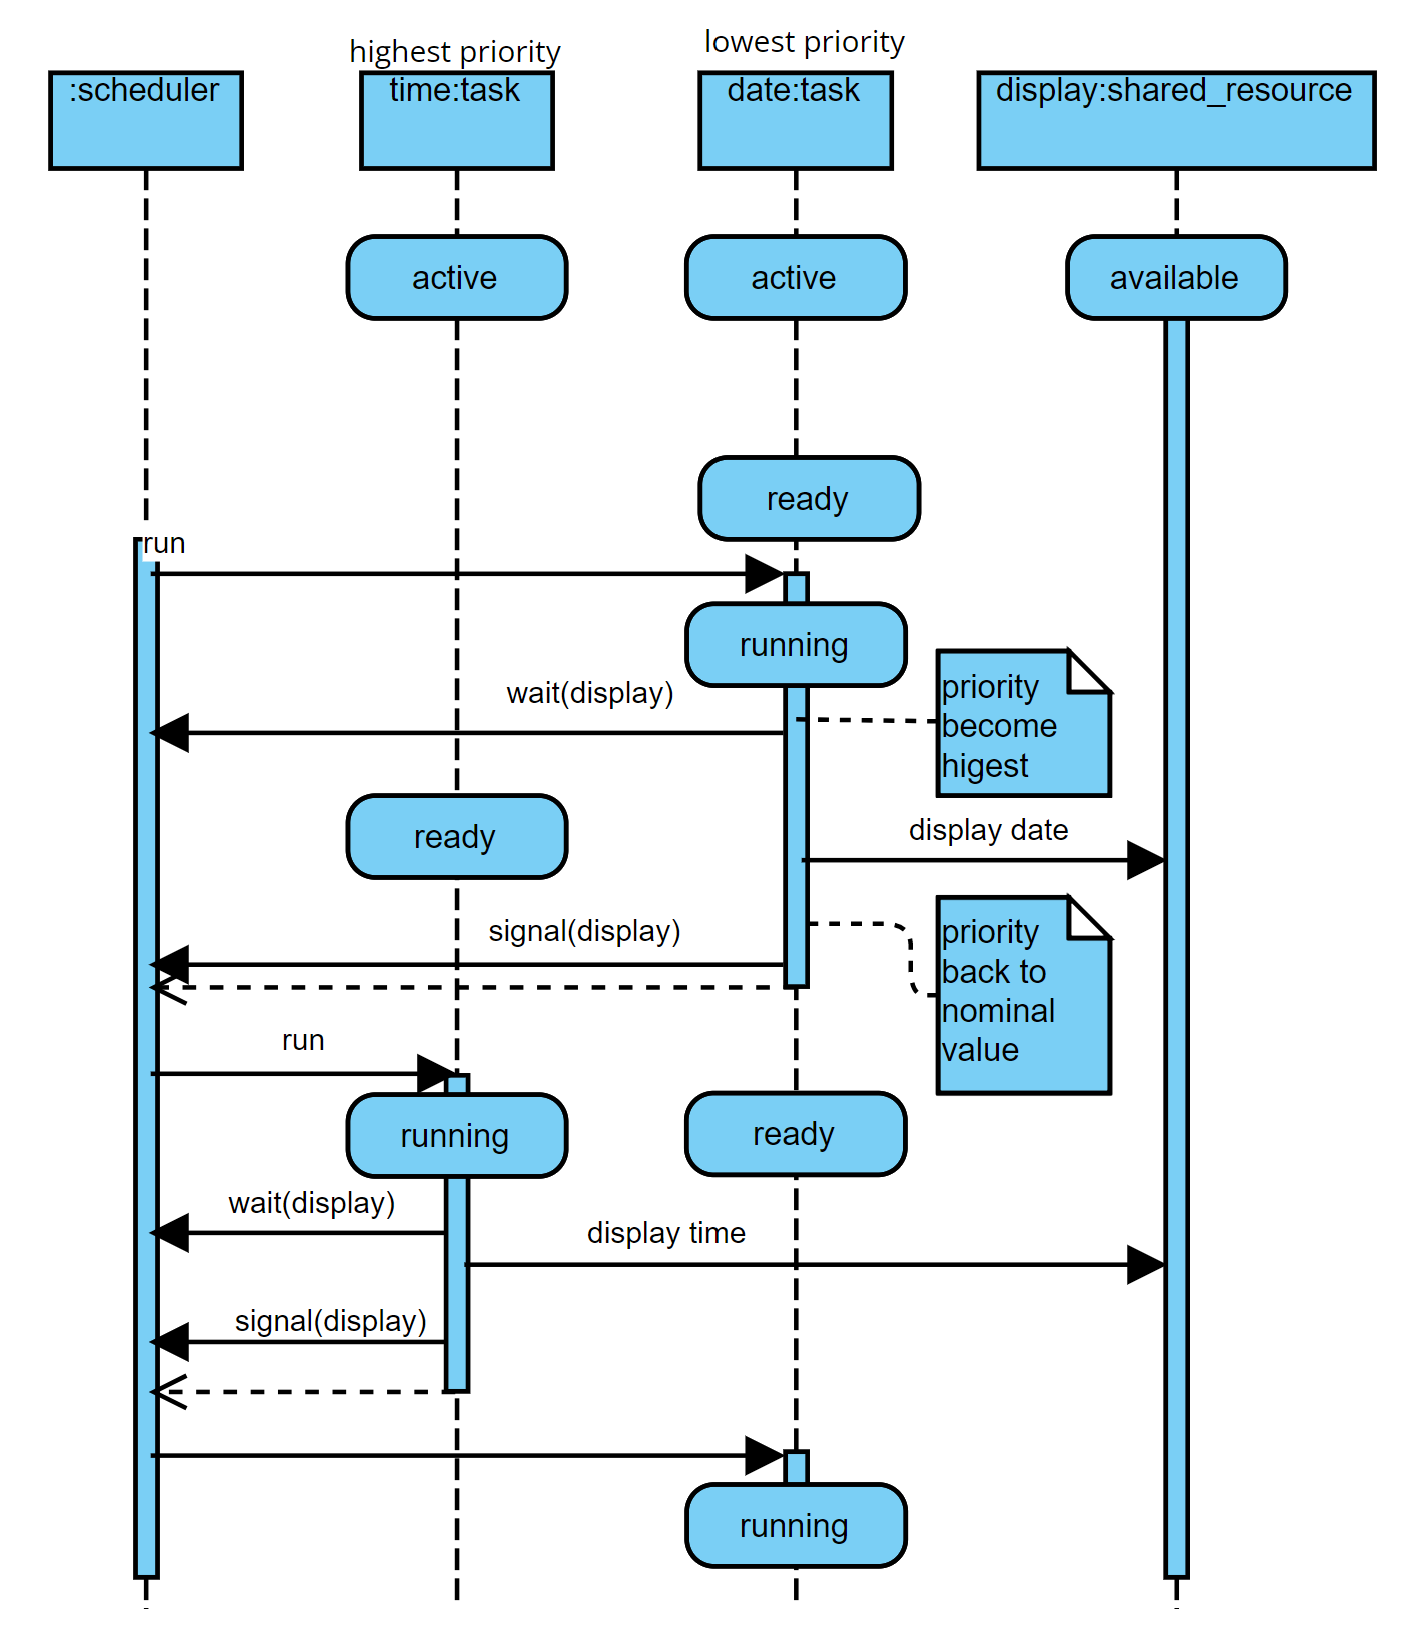
\includegraphics[width=0.5\textwidth]{sample_model_with_npp.png}
    \caption{Sample Model with Non-Preemptive Protocol }
    \label{fig:sample_model_with_npp}
\end{figure}


\subsection{Problem Arise}

As shown in ``Fig. \ref{fig:Example_in_which_NPP_causes_unnecessary_blocking_on_T1}'', this protocol will block the highest priority task $ \tau_{1} $ even though the task will not access the resource because the priority of the task $\tau_{3}$ has been increased to the maximum.

\begin{figure}[ht]
    \centering
    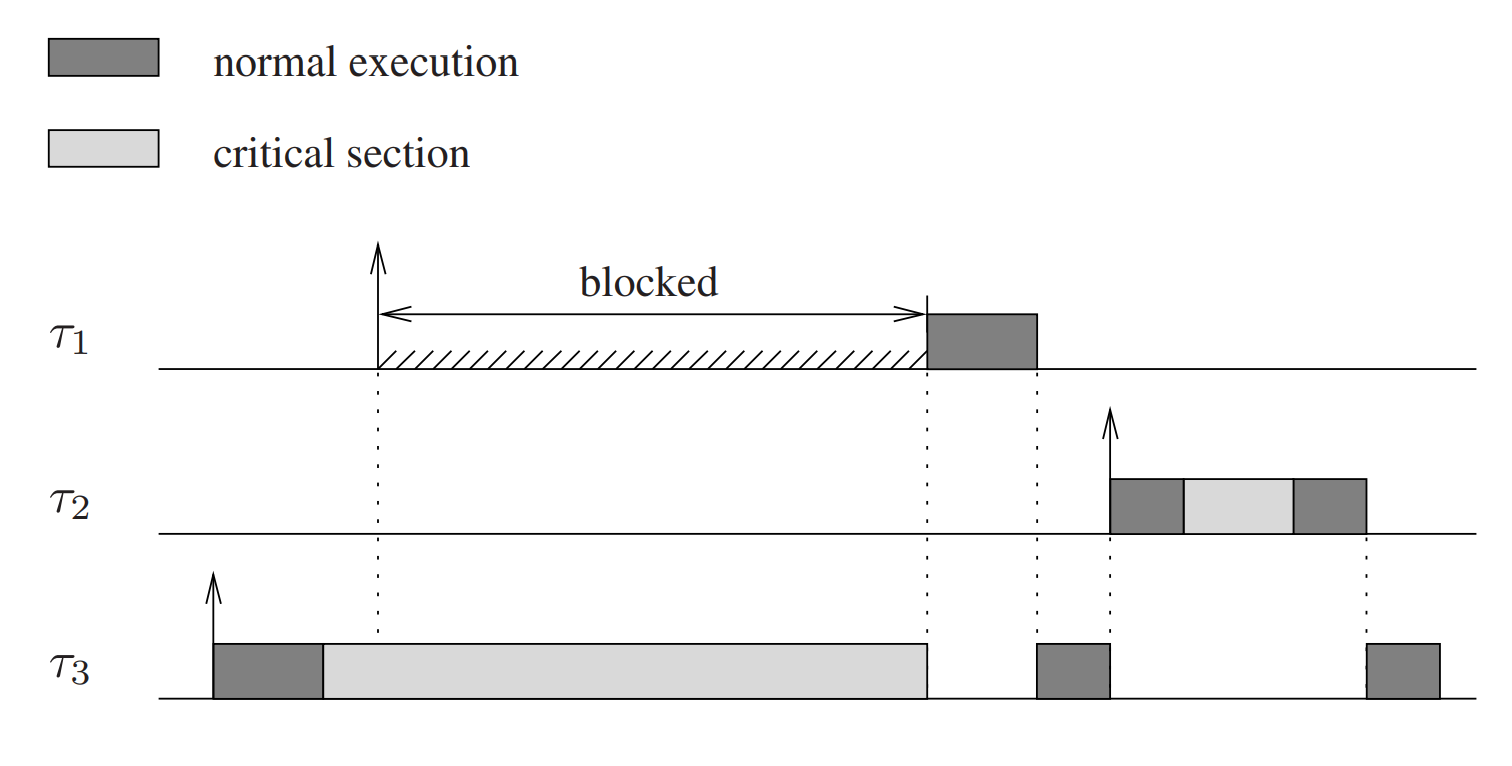
\includegraphics[width=0.5\textwidth]{Example_in_which_NPP_causes_unnecessary_blocking_on_T1}
    \caption{Example in which NPP causes unnecessary blocking on $ \tau_{1} $ \cite{b5}}
    \label{fig:Example_in_which_NPP_causes_unnecessary_blocking_on_T1}
\end{figure}

Back to our sample model, this situation can be illustrated by adding a new task that didn't use the resource,$ R_{d}$ like alarm task, $\tau_{a}$ as shown in ``Fig. \ref{fig:sample_model_problem_npp}''.

 
\begin{figure}[ht]
    \centering
    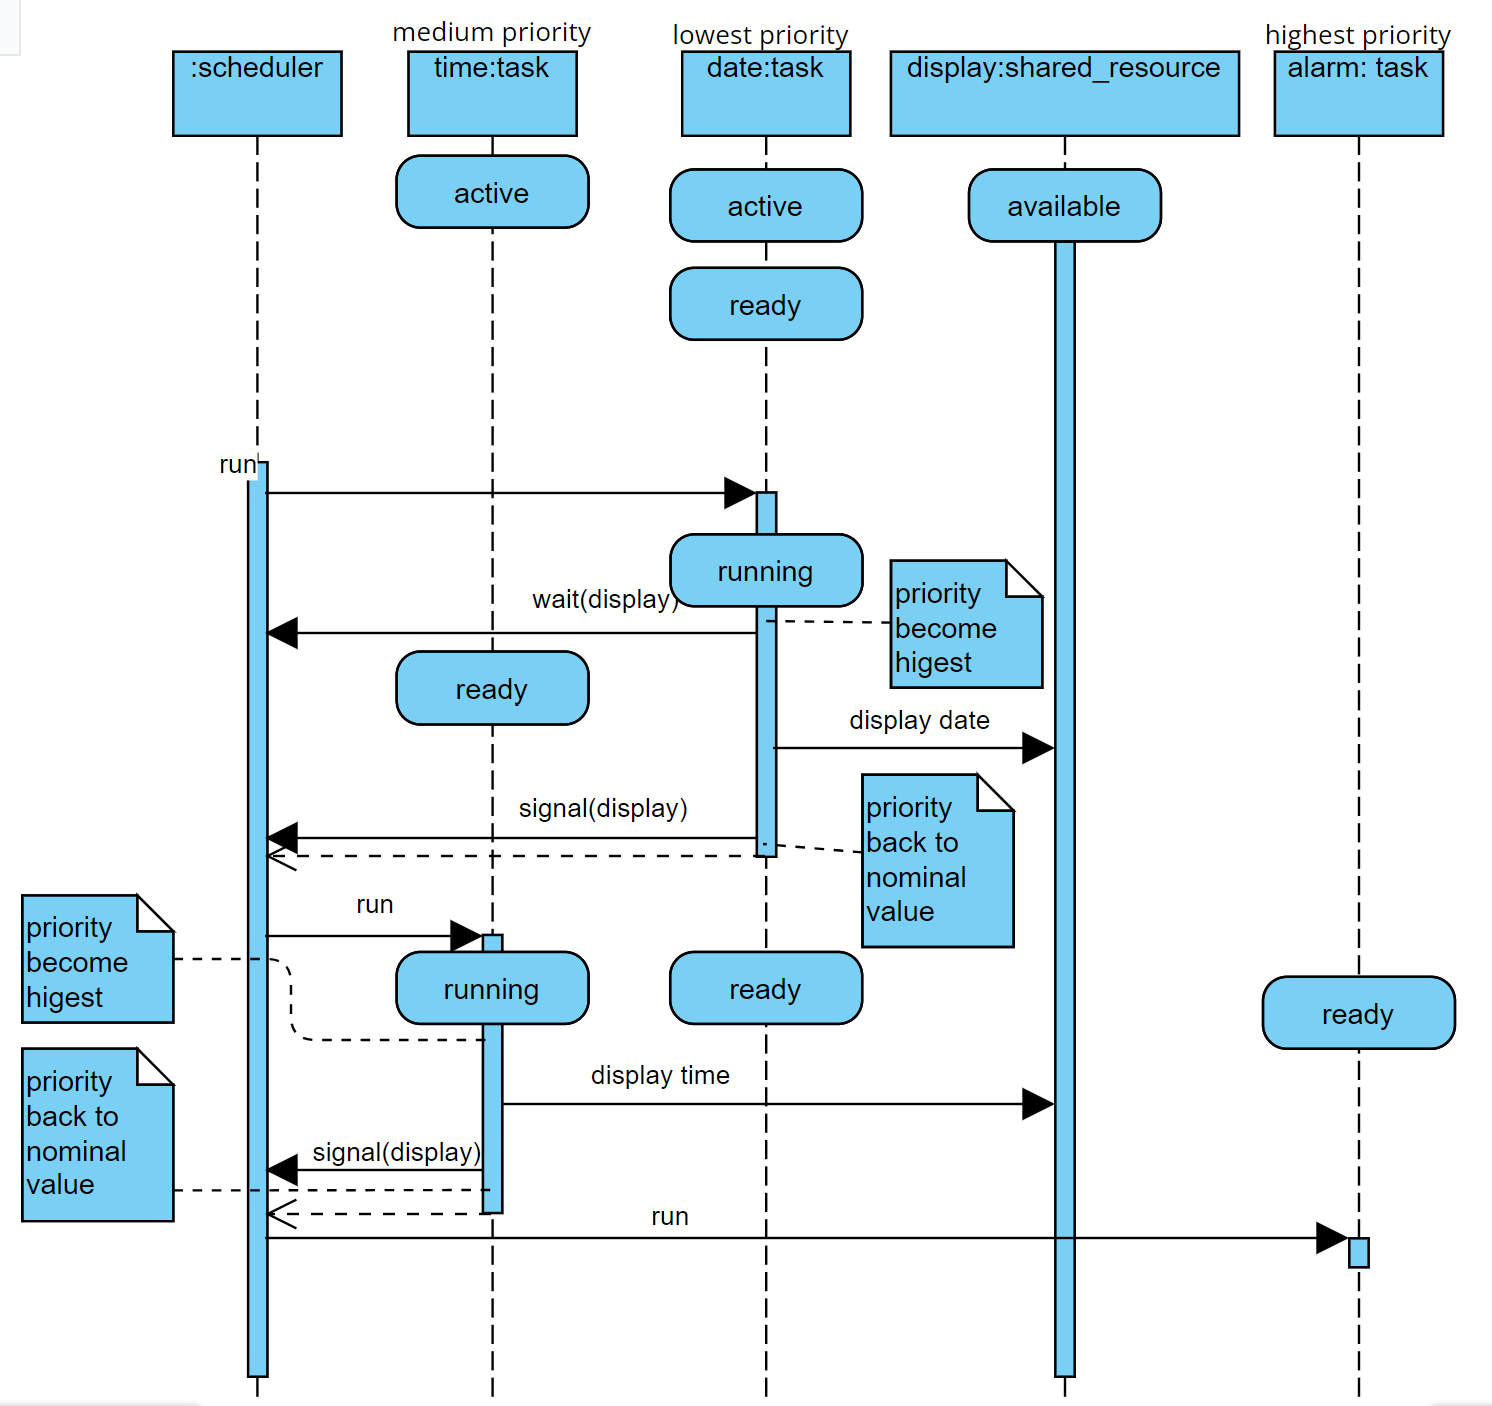
\includegraphics[width=0.5\textwidth]{sample_model_problem_npp}
    \caption{An Example in which NPP causes unnecessary blocking on alarm task, $ \tau_{a} $ }.
    \label{fig:sample_model_problem_npp}
\end{figure}

 This problem could be solved by the protocol in the next section, which is Highest Locker Priority (HLP) protocol.